\section{Patient level analysis}
\label{cascade-sec:patientLevel}
In this section I will outline the work performed for each patient and highlight work specifically done for certain patients due to their unique clinical features. However most of the analysis is streamlined and the workflow applied the same way to each patient. The following sections expand on the individual steps.
\begin{enumerate}
\item \textbf{Quality control:} Each sample of a patient is checked for kinship and sequencing quality
\item \textbf{Read mapping}
\item \textbf{Joint somatic variant calling:} SNPs, InDels and SVs are called jointly
\item \textbf{Copy number calling}
\item \textbf{Variant effect annotation:} short and structural variants are annotated with possible biological effects
\item \textbf{Phylogenetic reconstruction}
\item \textbf{Clonal deconvolution}
\end{enumerate}

\subsection{Analysis workflow}
\label{cascade-sec:workflow}
This section summarises the primary analysis performed for each patient in detail. Specific analysis, like RNA analysis are discussed in the individual patient sections. 

\subsubsection{Quality control}
\label{cascade-sec:qc}
When multiple samples per patient are available, the possibility of sample mix-ups and issues is higher than when just dealing with a tumour normal pair, so in addition to the standard read depth, sequencing quality and reads-on-target analysis that is routinely performed after sequencing, we performed an additional step of kinship detection. We use concepts commonly employed in germline cohort analysis, like child and parents (trio) or even large databases (gnomAD). As most germline variants are due to mendelian inheritance, we can use the percentage of shared homo- and heterozygous germline variants to estimate the relatedness of two samples. For our analysis we used NGSCheckMate \cite{Lee2017} and all the results shown in later sections are based on it, however we also used Somalier \cite{Pedersen2020} on two patient samples with surprising kinship results but Somalier confirmed the result.

While this analysis is very useful to detect samples which do not belong to a patient, either through mislabelling or similar, it does not protect from mix-ups within a patients samples. However nothing but orthogonal validation will be able to discern these errors.

Other quality controls were performed with fastQC \cite{Andrews2010} for read integrity and \lq\emph{CollectWgsMetrics}\rq~from Picard \cite{Picard2018} for WGS samples and \lq\emph{samtools flagstat}\rq~\cite{Danecek2021} for on-target estimation for WES samples.

\subsubsection{Read mapping}
\label{cascade-sec:mapping}
For highest mapping performance, reads were aligned alternative contig aware with BWA~\cite{Li2013} (v0.7.17)  to GRCh38 (\emph{GCA\_000001405.15}) with alternative contigs but no decoy regions. Initial mapping was post-processed with \lq\emph{bwa-postalt.js}\rq~from bwa-kit to adjust the mapping assignment and quality mapping both to alternative and canonical contigs. Finally reads were duplicate marked with \lq\emph{MarkDuplicates}\rq~from the Picard-toolkit.

\subsubsection{Joint somatic variant calling}
\label{cascade-sec:jsvc}
For short variants (SNPs and InDels), the workflows presented in \autoref{ch:variantcalling} were used and while the Strelka2Pass workflow generates structural variants calls, they are not jointly called over all samples. Instead for the structural variants (SVs) we used GRIDSS2 \cite{Cameron2021}, which has a calling model for multiple related tumour samples and as GRIDSS2 is also a prerequisite for copy number calling with PURPLE (\autoref{cascade-sec:cnv}) using the same structural variants allows a higher conformity of analysis.


\subsubsection{Copy number analysis}
\label{cascade-sec:cnv}
After somatic variant calling, copy number analysis is a stable when dissecting the resistance and driver alterations of a tumour sample. While lung cancers are known for their high mutational burden \cite{Alexandrov2020}, often genetic amplifications can be found as driver or resistance mechanism. One of the more common resistance mechanisms is a high \textit{EGFR} or \textit{MET} amplification which significantly affect transcription \cite{Bjaanaes2021}. And while copy number alterations are often shared between metastases \cite{Ni2013}, the same heterogeneity that can be found in variant calling analysis also affects copy number analysis. Many modern copy number calling method will use the B-allele frequency , the allele frequency of a heterozygous germline variant, to gain allele specific copy number calls \cite{Favero2015,Talevich2016,Cameron2019a}. However each of those methods will only use the input of one tumour and one germline sample, very similar to \autoref{ch:variantcalling} we can actually improve the performance by analysing all tumour samples jointly. So far only HATCHet \cite{Zaccaria2020} has a joint copy number calling method.

\todo[inline]{Explain why we didnt use hatchet in the end? subjective parameter tuning?}
\todo[inline]{Explain purple vs sequenza for WGS vs WES}

\subsubsection{Variant effect annotation}
\label{cascade-sec:vep}

\subsubsection{Phylogenetic reconstruction}
\label{cascade-sec:phylo}

\subsubsection{Clonal deconvolution}

\subsection{Patient CA-A}
\label{cascade-sec:CA99}

This patient was a 61 year old male  with a metastatic \textit{RET-KIF5B} fusion positive NSCLC. After failure of Carboplatin, Pemetrexed, and Pembrolizumab as well as Lenvatinib, with compassionate access to Selpercatinib (\autoref{fig:ca99timeline}) he experienced almost immediate improvement with decreased levels of carcinoembryonic antigen and almost 100\% reduction of fusion positive ctDNA after one month (\autoref{fig:ca99ctDNA}). Similar to the ctDNA analysis, Positron emission tomography-computed tomography imaging revealed significantly reduced tracer uptake in multiple sites and partial response (\autoref{fig:ca99pet}.

\begin{figure}[!ht]
\centering
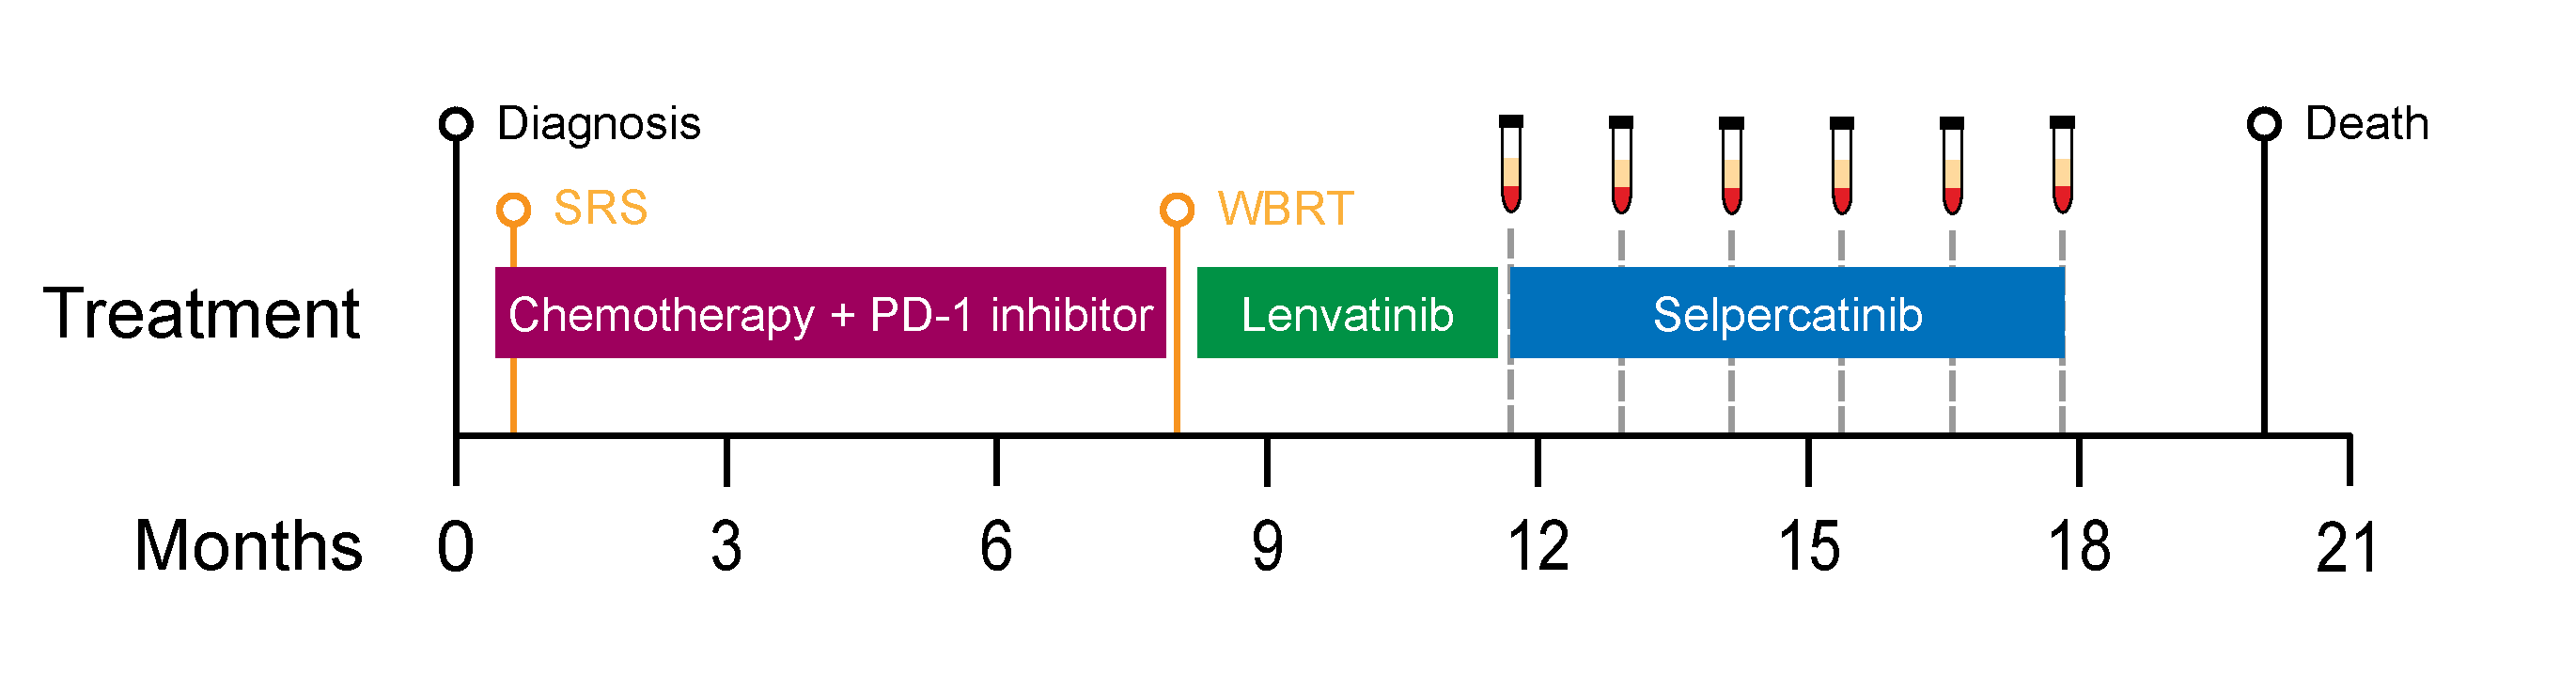
\includegraphics[width=.99\linewidth]{Figures/CA-A_timeline}
\caption[Timeline of patient CA-A from diagnosis until death]{Timeline of patient CA-A from diagnosis until death: Diagnostic biopsy detected \textit{KIF5B-RET} positive lung adenocarcinoma; SRS: stereotactic radiosurgery; WRBT: whole brain radiation therapy; a total of six blood samples were taken just before and during the selpercatinib treatment.} \label{fig:ca99timeline}
\end{figure}


Serial sampling of the plasma of the patient revealed the previously undetected RET~G810S resistance mutation after three moths of treatment . While at this point the driver mutation allele frequency was still dropping in the plasma, by month four the abundance of RET~G810S had increased and was accompanied by additional mutations in the same site (RET~G810R, C and V). In addition with the increase of fusion positive ctDNA this suggests that any mutation in this site affects the efficiency of Selpercatinib. While the patient initially was responsive to the treatment, repeat PET scans showed a progressive disease after six months, which ultimately lead to the death of the patient (\autoref{fig:ca99pet}).

\begin{figure}[!ht]
\centering
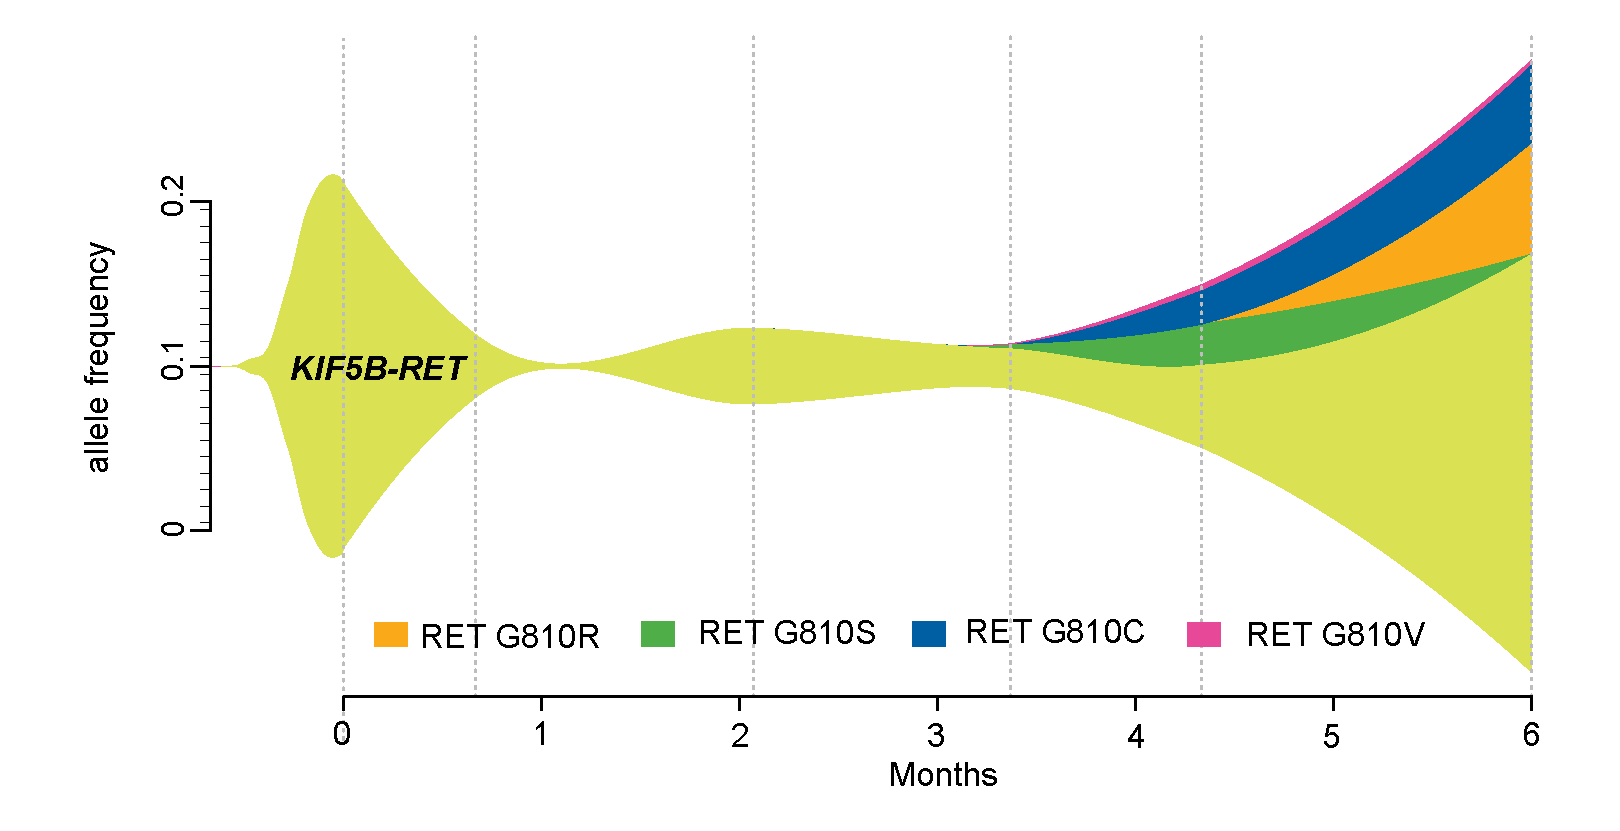
\includegraphics[width=.99\linewidth]{Figures/CA-A_ctDNAstream}
\caption[Allelic frequencies of of driver and emerging resistance mutations]{Allelic frequencies of of driver and emerging resistance mutations during Selpercatinib treatment (11 months after diagnosis); \textit{KIF5B-RET} fusion is the initiating driver with RET~G810R/S/C/V the emerging resistance SNPs} \label{fig:ca99ctDNA}
\end{figure}


\begin{figure}[!ht]
\centering
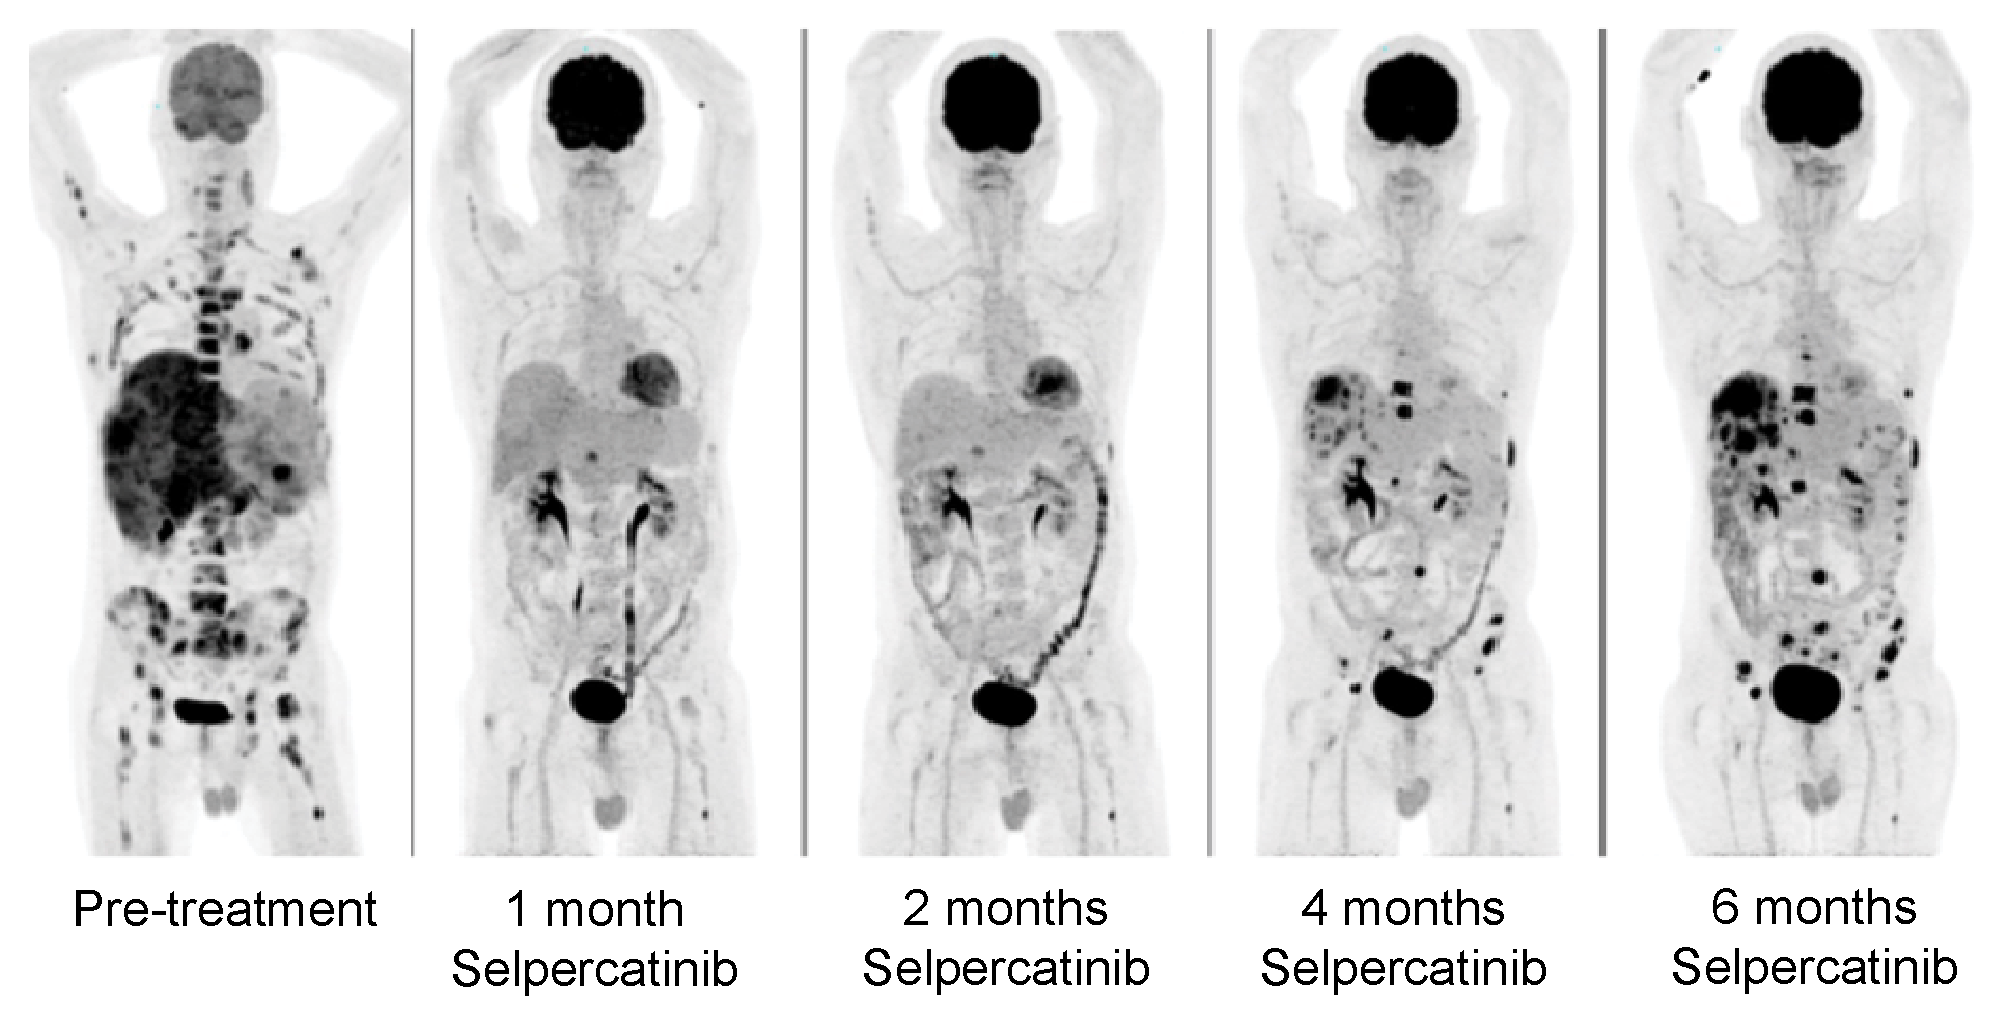
\includegraphics[width=.99\linewidth]{Figures/CA-A_PETscans}
\caption[PET scans of patient CA-A before and during Selpercatinib treatment]{PET scans of patient CA-A before and during Selpercatinib treatment} \label{fig:ca99pet}
\end{figure}


\begin{figure}[!ht]
\centering
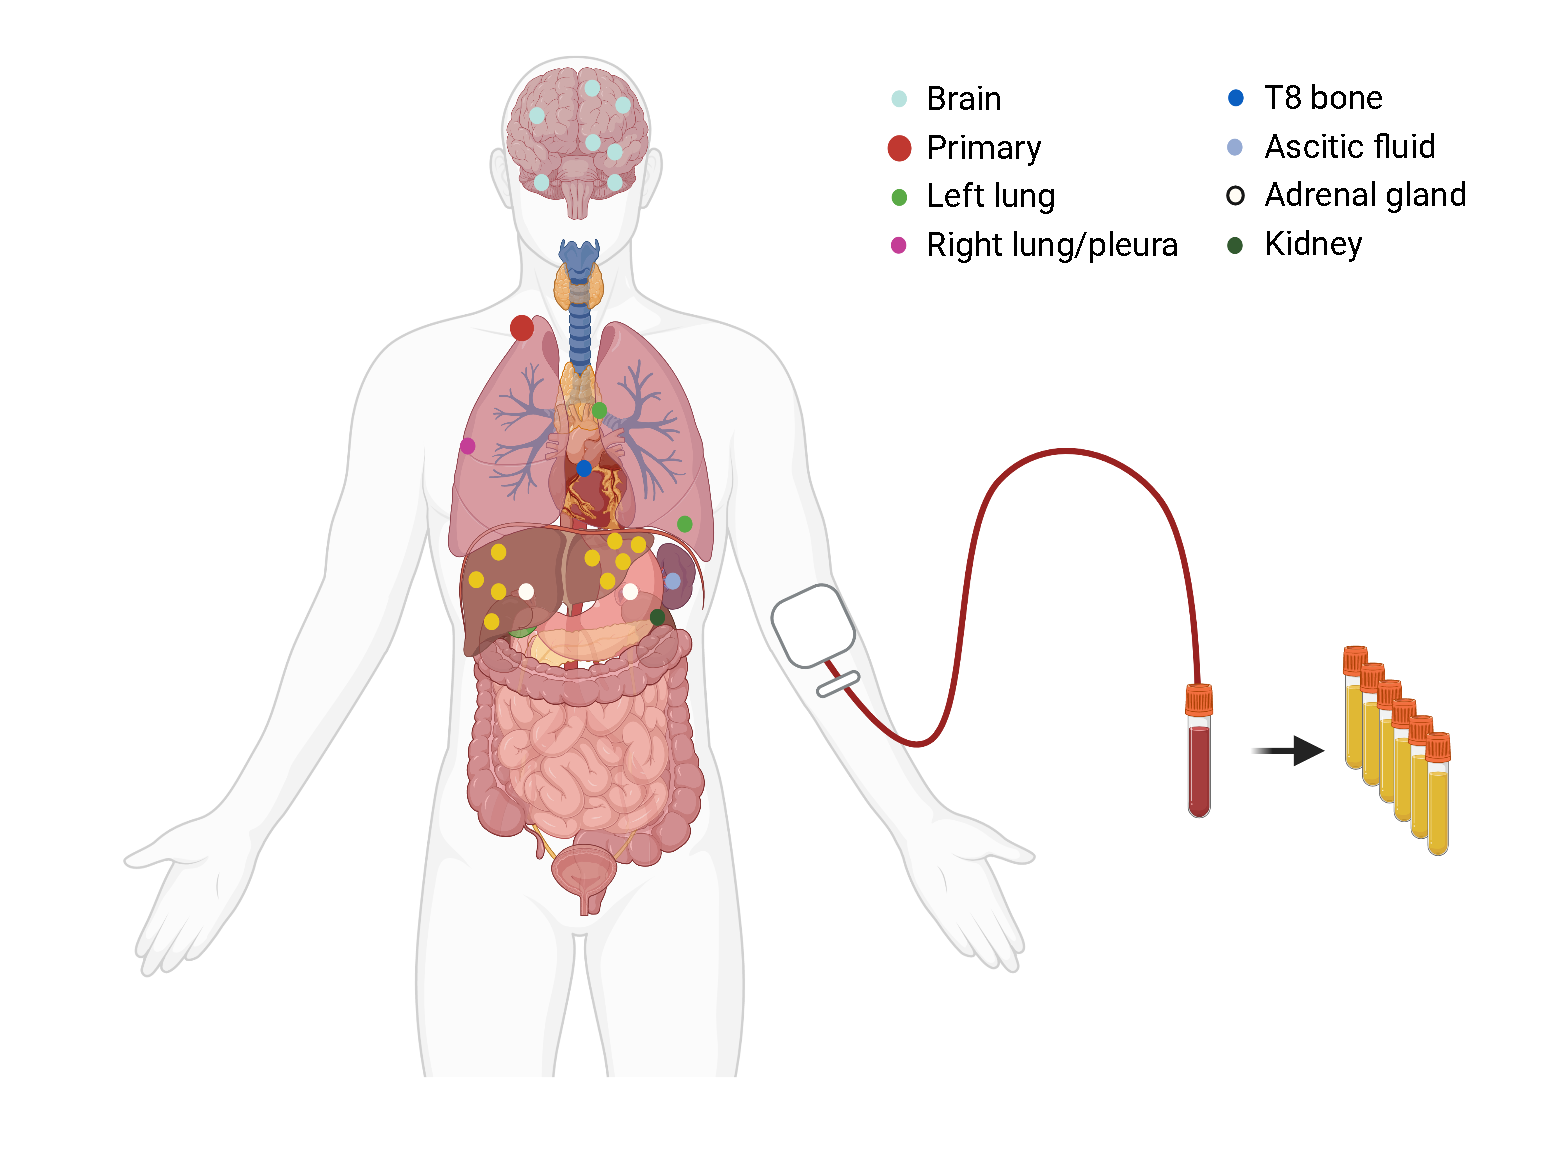
\includegraphics[width=.99\linewidth]{Figures/CA-A_schematic_CA99_organColours}
\caption[Schematic of analysed tumour lesions in patient CA-A]{Schematic of analysed tumour lesions in patient CA-A: Primary diagnostic sample shown in red; sequenced autopsy samples shown in green (8); and bio banked samples shown in blue (16). plasma tubes depict five serial samples taken during treatment and one at autopsy} \label{fig:ca99schematic}
\end{figure}


At autopsy, 24 tumour tissue biopsies and a post mortem blood sample were collected and eight of them were selected for WGS at 130x coverage (\autoref{fig:ca99schematic}). 

%we clear all floats before we go to the next patient
\cleardoublepage

\subsection{Patient CA-I}
\label{cascade-sec:CA51}



\begin{figure}[!ht]
\centering
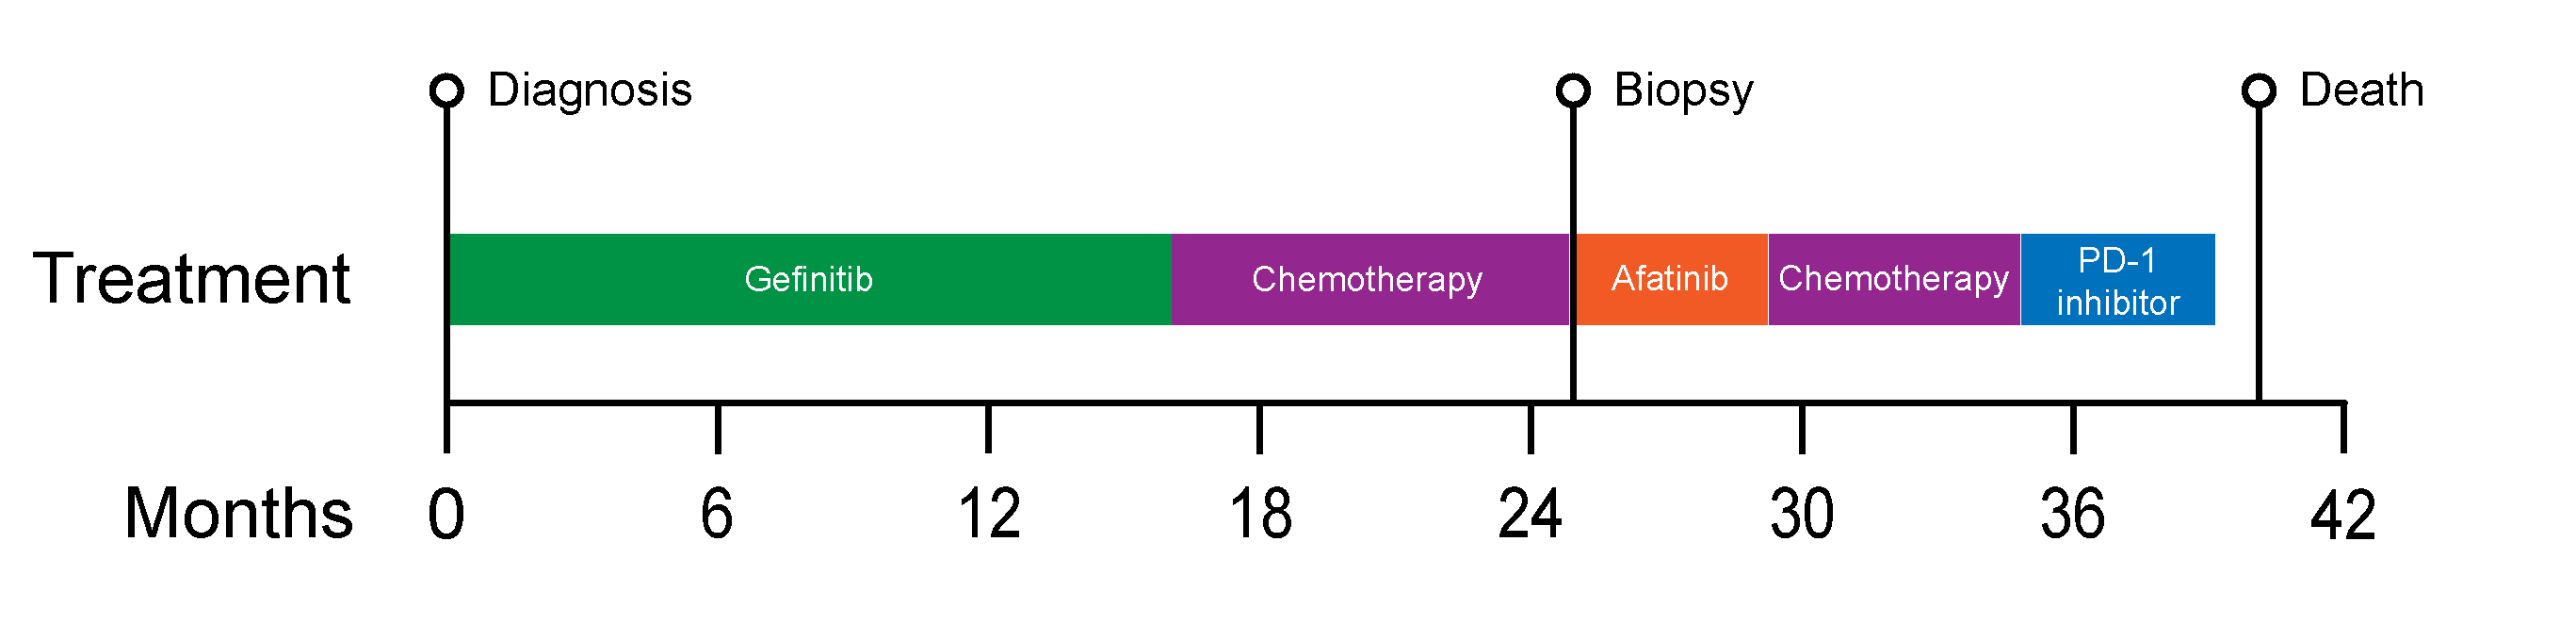
\includegraphics[width=.99\linewidth]{Figures/CA-I_timeline}
\caption[Timeline of patient CA-I from diagnosis until death]{Timeline of patient CA-I from diagnosis until death: Diagnostic biopsy detected EGFR exon 19 deletion lung adenocarcinoma; Second biopsy after 24 months revealed additional EGFR~T790M mutation and small cell transformation} \label{fig:ca51timeline}
\end{figure}



\begin{figure}[!ht]
\centering
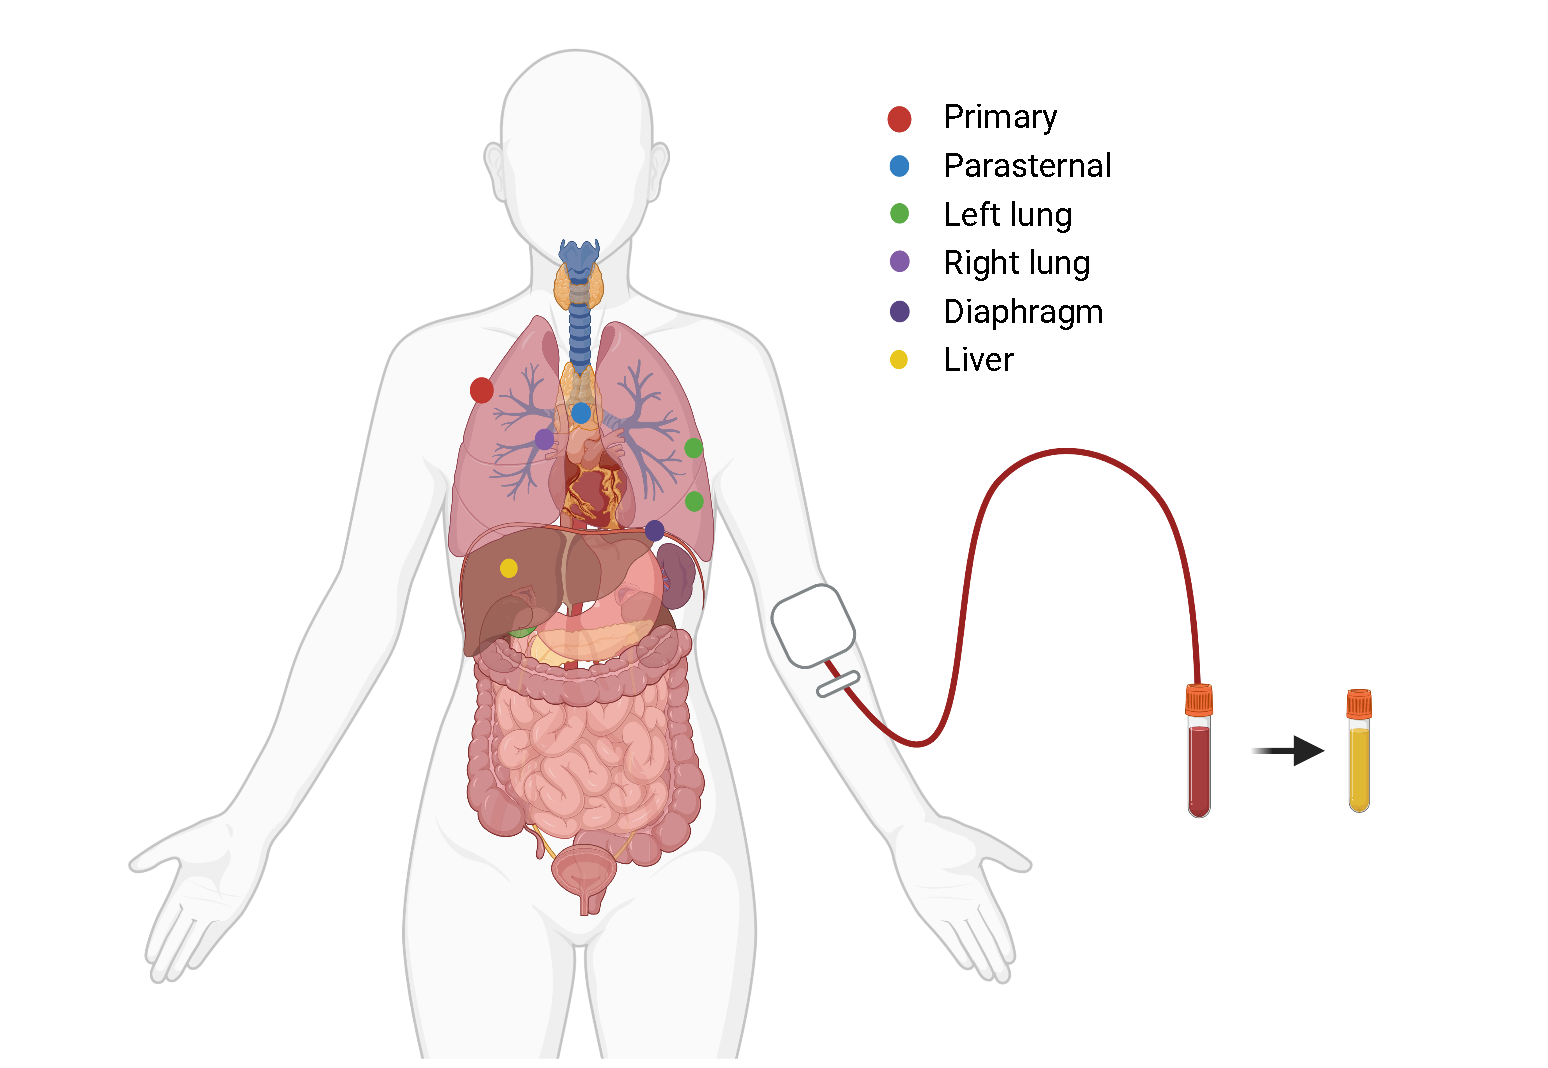
\includegraphics[width=.99\linewidth]{Figures/CA-I_schematic_CA51_organColours}
\caption[Schematic of analysed tumour lesions in patient CA-I]{Schematic of analysed tumour lesions in patient CA-I: Primary diagnostic sample shown in red; sequenced autopsy samples shown in green (6). Right side shows one post mortem blood sample taken} \label{fig:cas51schematic}
\end{figure}


%we clear all floats before we go to the next patient
\cleardoublepage

\subsection{Patient CA-J}
\label{cascade-sec:CA80}


\begin{figure}[!ht]
\centering
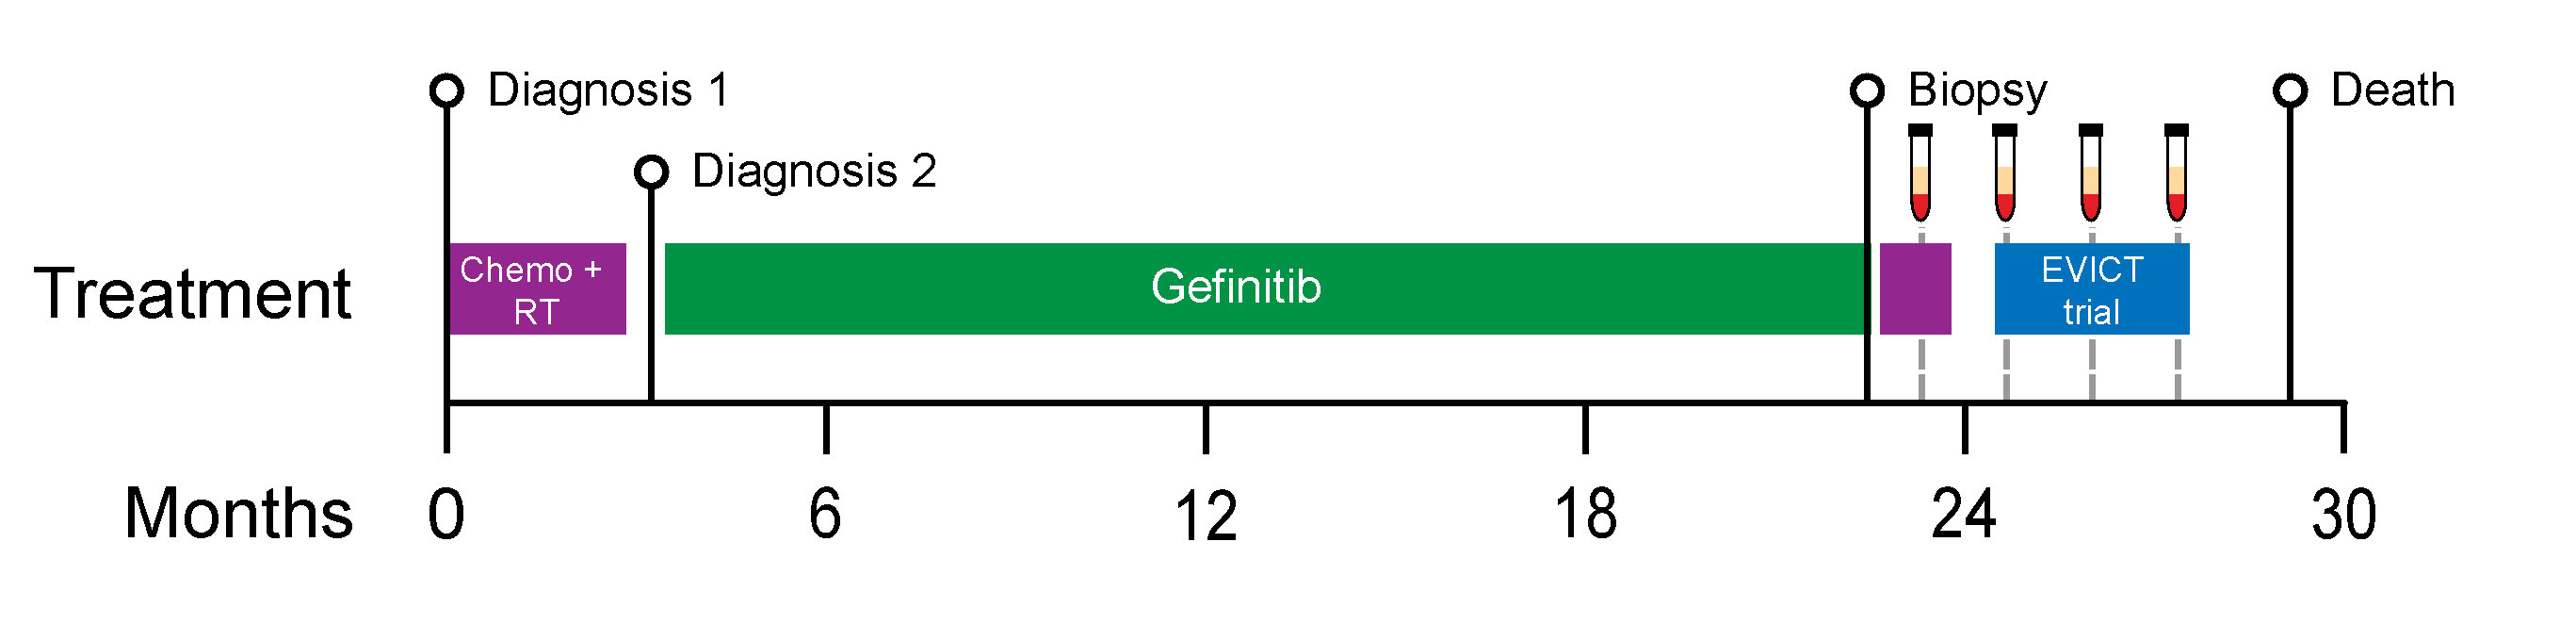
\includegraphics[width=.99\linewidth]{Figures/CA-J_timeline}
\caption[Timeline of patient CA-J from diagnosis until death]{Timeline of patient CA-J from diagnosis until death: Diagnostic biopsy detected EGFR~L858R positive stage IIIB lung adenocarcinoma; Second diagnosis after 3 months revealed additional brain and lung metastasis with a reclassification to stage IV; Biopsy at the end of erlotinib treatment revealed additional BRAF~V600E mutation; one blood sample was taken during the second round of chemotherapy and three more during the time the patient was enrolled in the EVICT trial} \label{fig:ca80timeline}
\end{figure}





\begin{figure}[!ht]
\centering
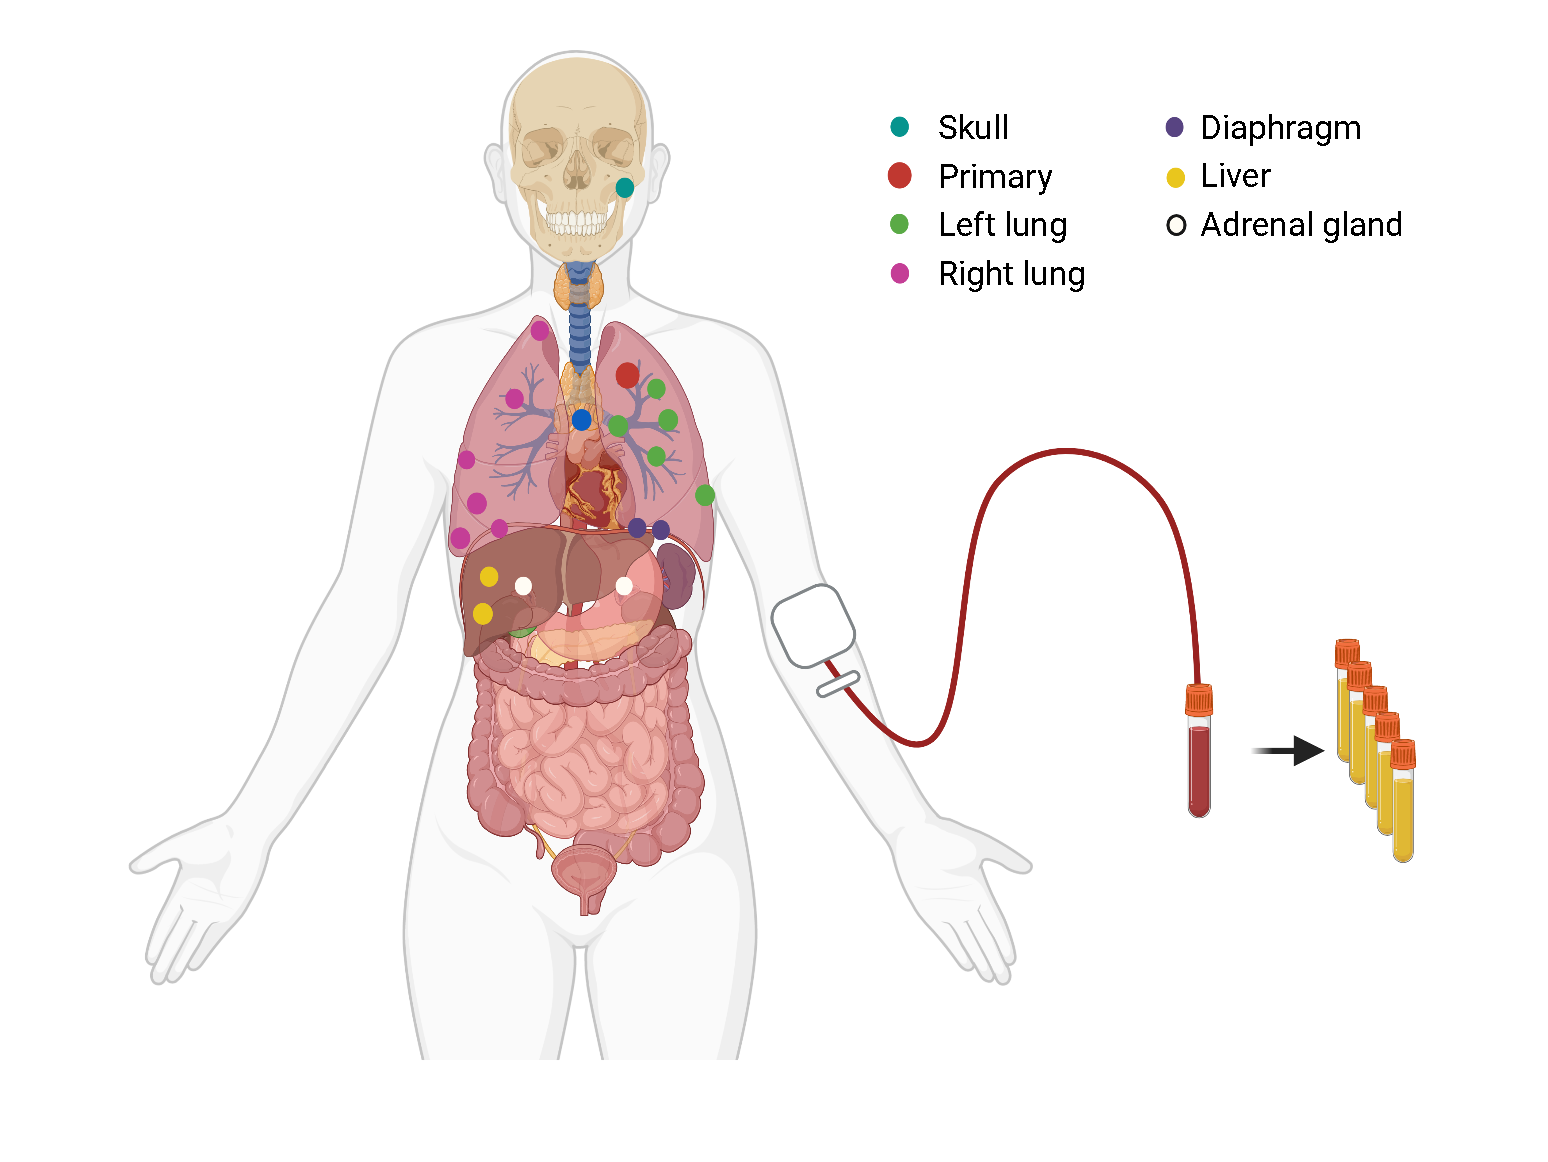
\includegraphics[width=.99\linewidth]{Figures/CA-J_schematic_CA80_organColours}
\caption[Schematic of analysed tumour lesions in patient CA-J]{Schematic of analysed tumour lesions in patient CA-J: Primary diagnostic sample shown in red; sequenced autopsy samples shown in green (5); and bio banked samples shown in blue (14). plasma tubes depict four serial samples taken during treatment and one at autopsy} \label{fig:cas80schematic}
\end{figure}


%we clear all floats before we go to the next patient
\cleardoublepage

\subsection{Patient CA-K}
\label{cascade-sec:CA82}

\begin{figure}[!ht]
\centering
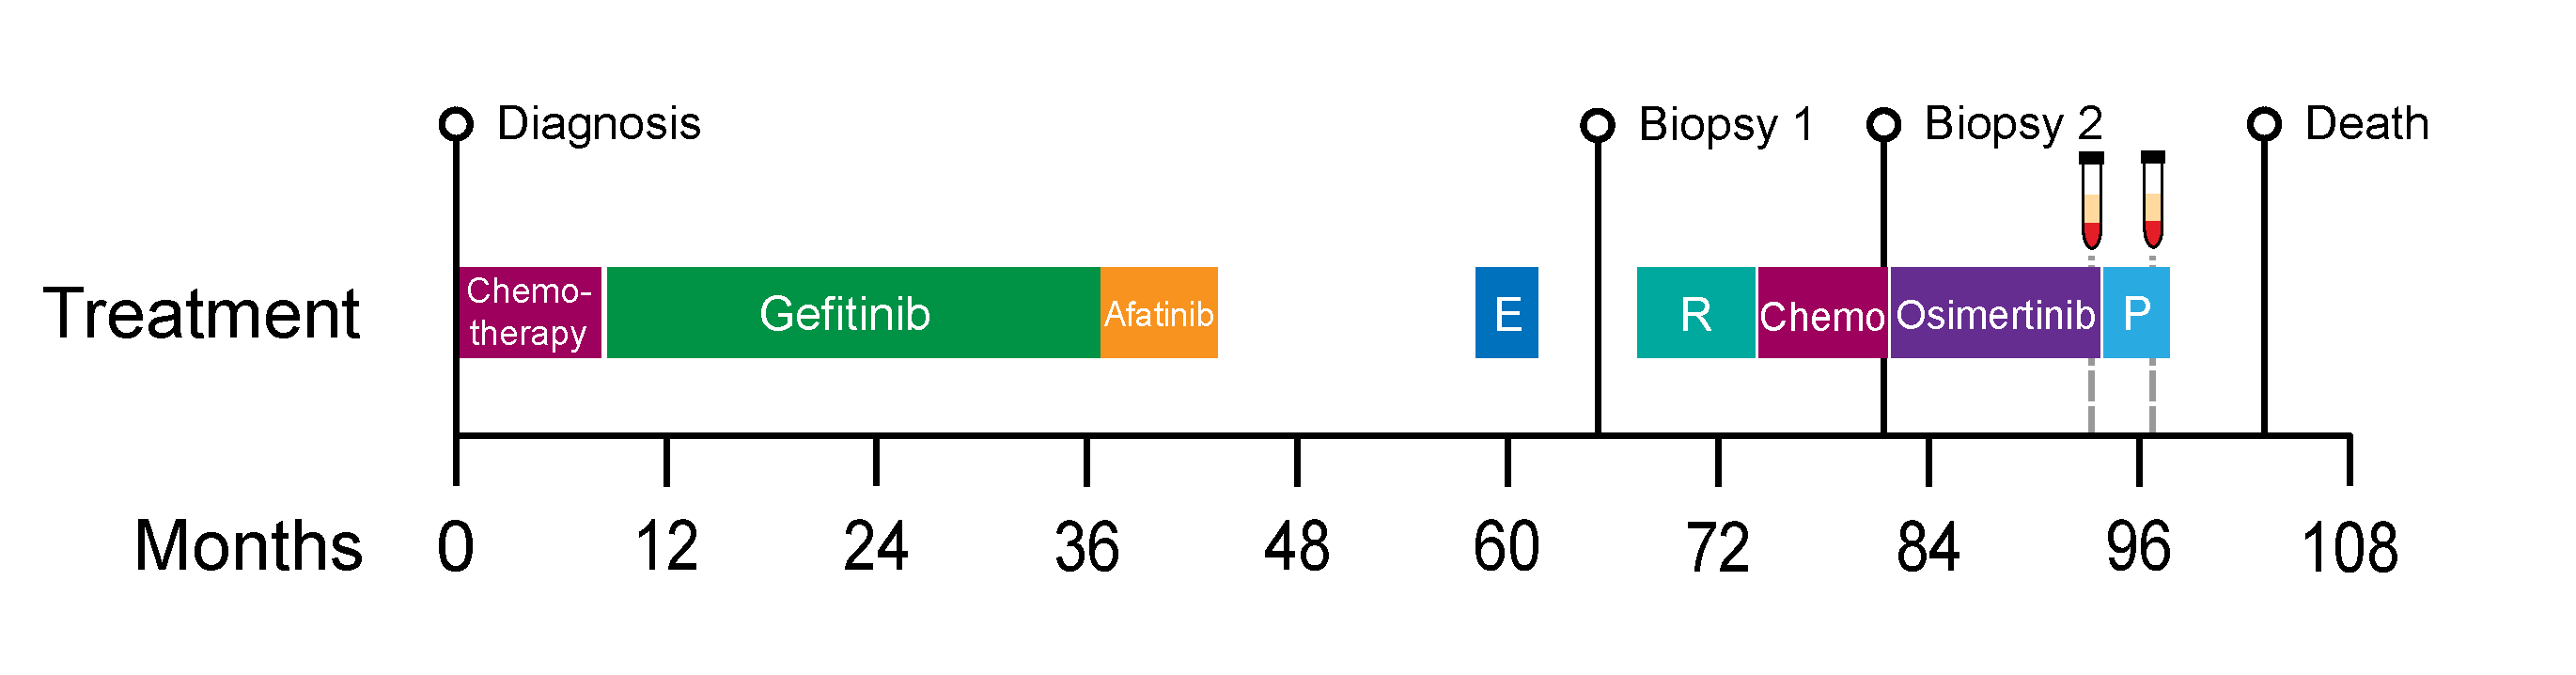
\includegraphics[width=.99\linewidth]{Figures/CA-K_timeline}
\caption[Timeline of patient CA-K from diagnosis until death]{Timeline of patient CA-K from diagnosis until death: Diagnostic biopsy detected EGFR~L858R positive lung adenocarcinoma;  Biopsy 1 after 66 months showed additional EGFR~T790M mutation; Biopsy 2 showed no additional variants; one blood sample was taken towards the end of Osimertinib treatment and one second one during PD-1 checkpoint blockade treatment. E: Erlotinib; R: Rociletinib; P: PD-1 inhibitor} \label{fig:ca82timeline}
\end{figure}




\begin{figure}[!ht]
\centering
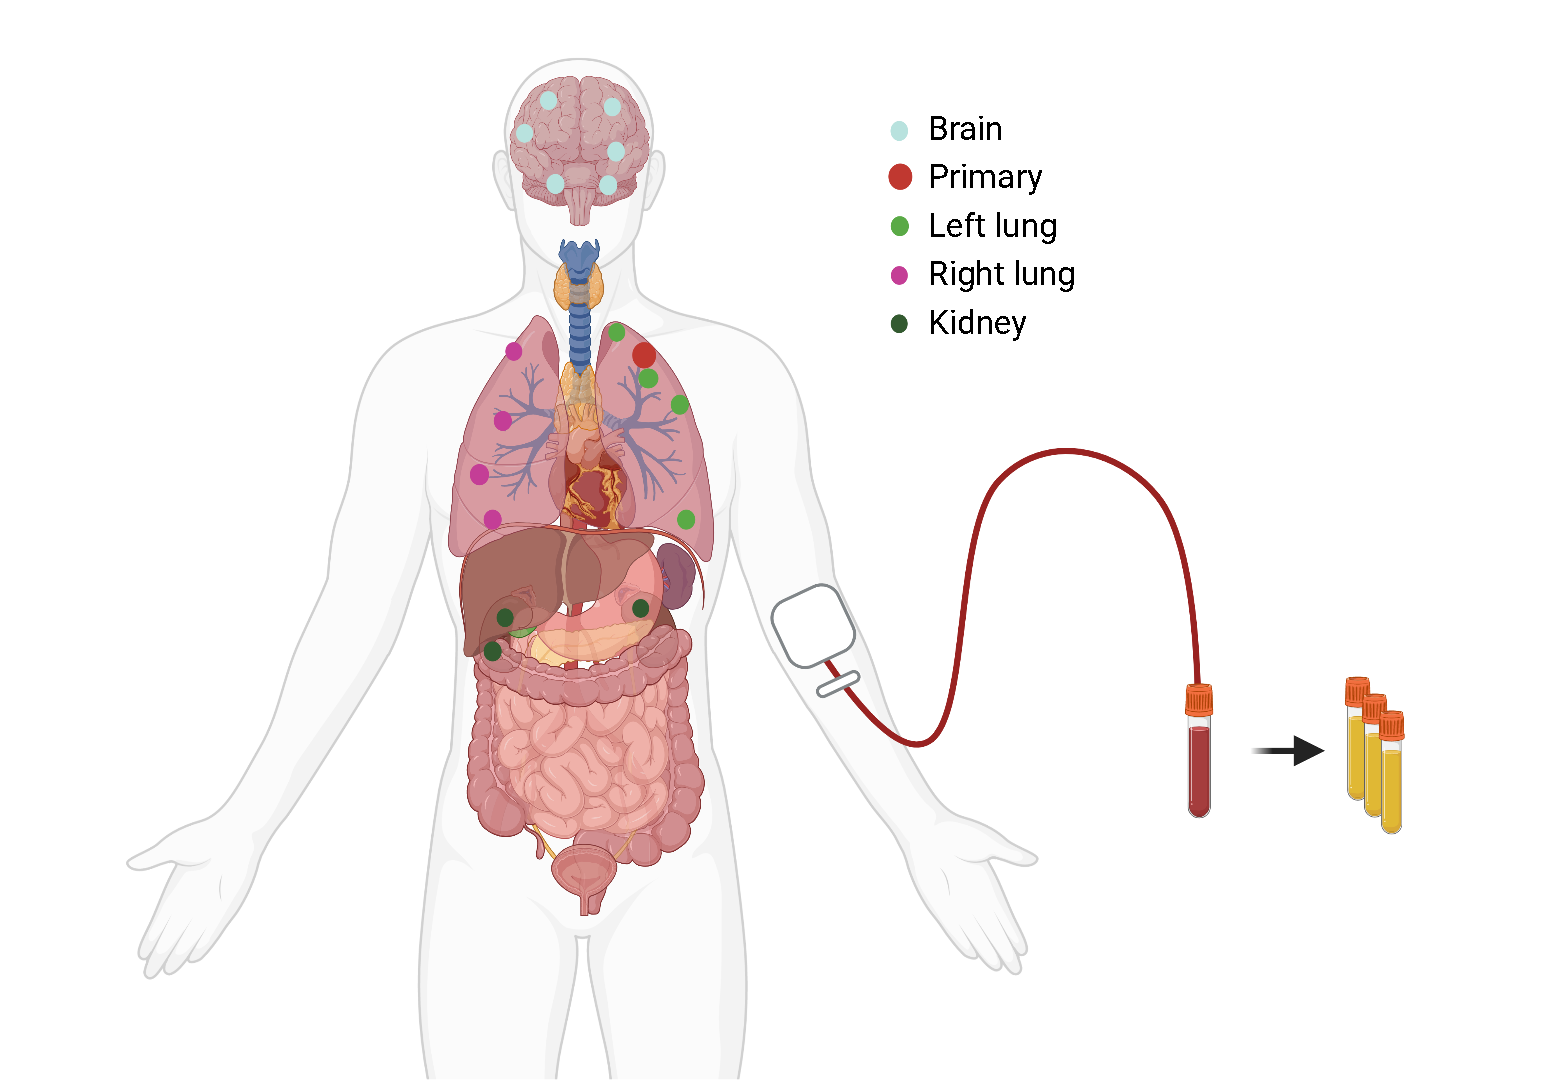
\includegraphics[width=.99\linewidth]{Figures/CA-K_schematic_CA82_organColours}
\caption[Schematic of analysed tumour lesions in patient CA-K]{Schematic of analysed tumour lesions in patient CA-K: Primary diagnostic sample shown in red; sequenced autopsy samples shown in green (6); and bio banked samples shown in blue (11). plasma tubes depict two serial samples taken during treatment and one at autopsy} \label{fig:cas82schematic}
\end{figure}

%we clear all floats before we go to the next patient
\cleardoublepage

\subsection{Patient CA-L}
\label{cascade-sec:CA86}


\begin{figure}[!ht]
\centering
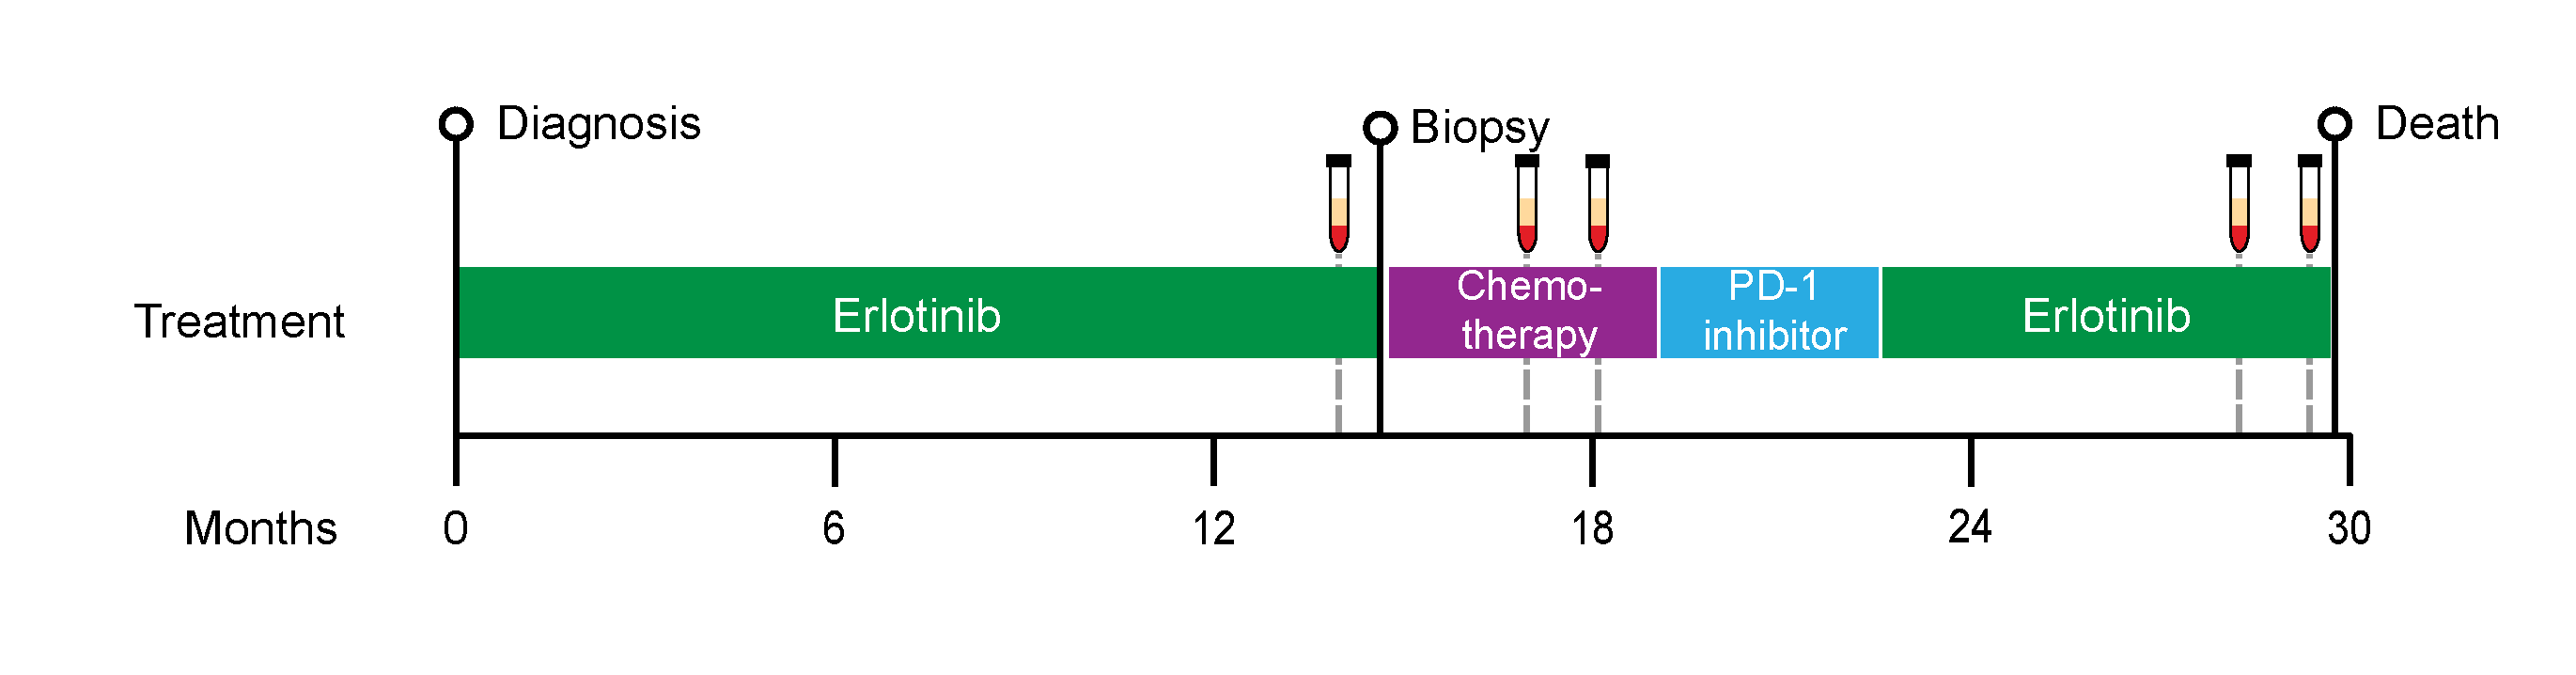
\includegraphics[width=.99\linewidth]{Figures/CA-L_timeline}
\caption[Timeline of patient CA-L from diagnosis until death]{Timeline of patient CA-L from diagnosis until death: Diagnostic biopsy detected EGFR exon 19 deletion positive lung adenocarcinoma;  Biopsy after 15 months Erlotinib treatment showed signs of small cell transformation; blood samples were taken at the end of the first Erlotinib treatment, during the chemotherapy treatment and  28 and 29 months after the initial diagnosis.} \label{fig:ca82timeline}
\end{figure}





\begin{figure}[!ht]
\centering
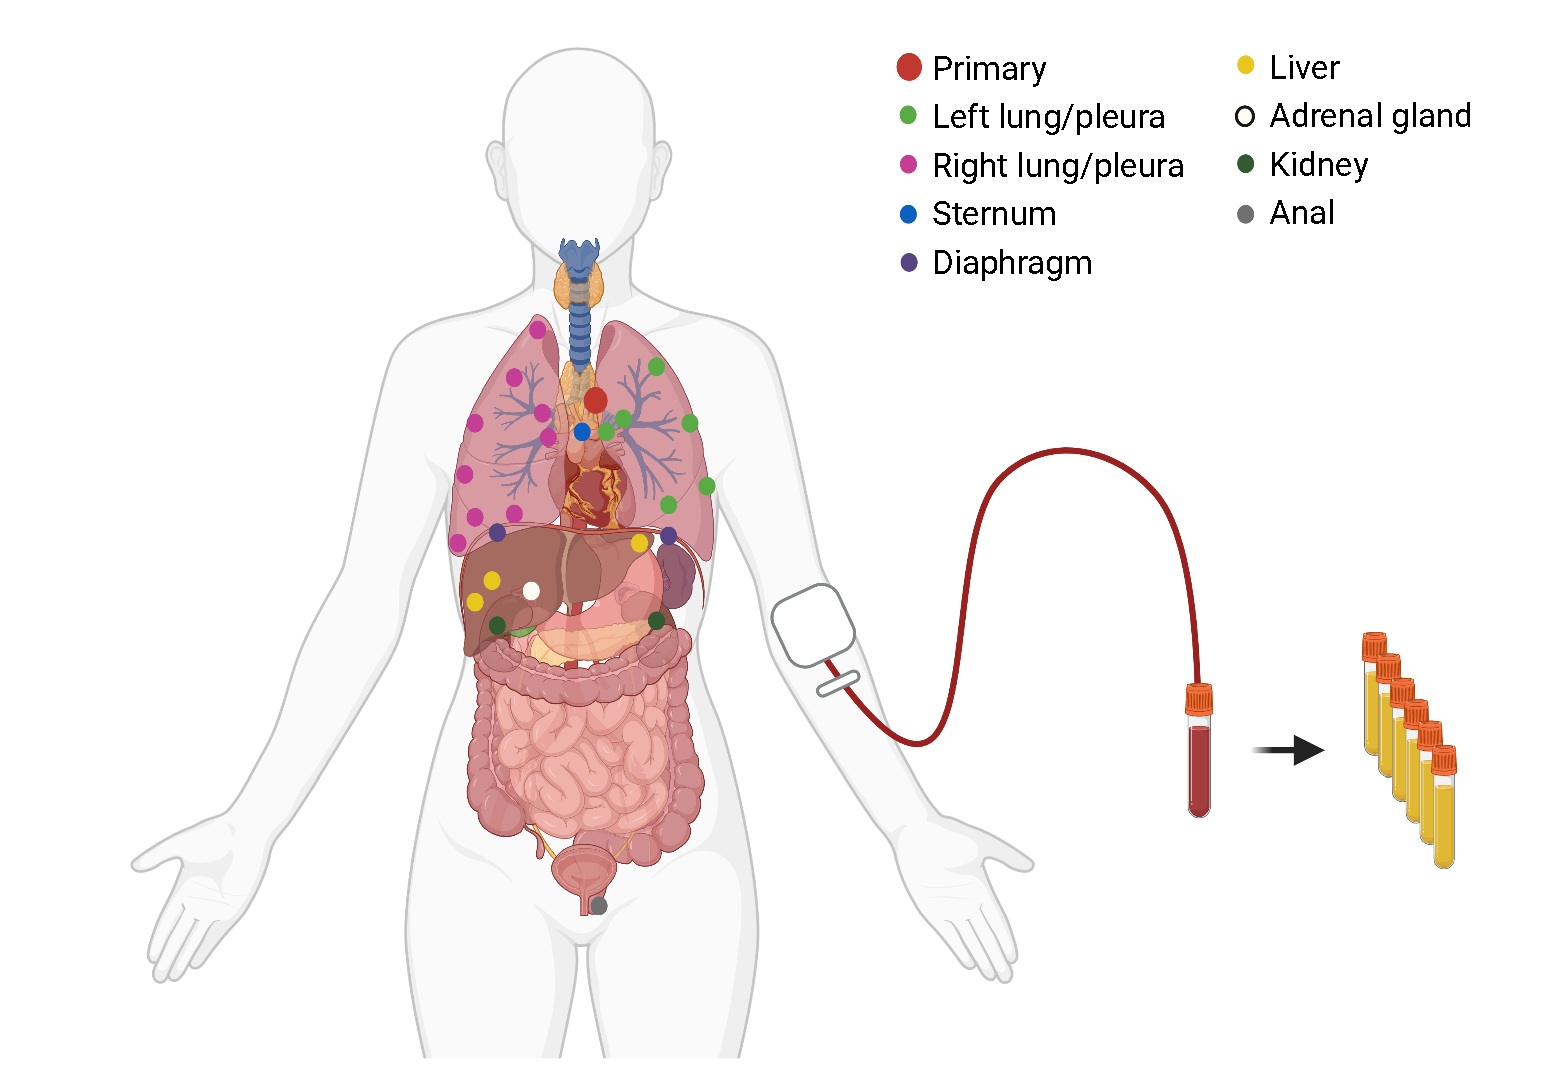
\includegraphics[width=.99\linewidth]{Figures/CA-L_schematic_CA86_organColours}
\caption[Schematic of analysed tumour lesions in patient CA-L]{Schematic of analysed tumour lesions in patient CA-L: Primary diagnostic sample shown in red; sequenced autopsy samples shown in green (4); and bio banked samples shown in blue (22). plasma tubes depict five serial samples taken during treatment and one at autopsy} \label{fig:cas86schematic}
\end{figure}



%we clear all floats before we go to the next section
\cleardoublepage

\section{Cohort level analysis}
\label{cascade-sec:cohortLevel}

\todo[inline]{short explanation about what this does}


\subsection{Phylogenetic reconstruction}
\label{cascade-sec:phylo}

\todo[inline]{Phylogenies and comparisons}